\documentclass[12pt]{article}
\usepackage[spanish]{babel}
\usepackage[utf8]{inputenc}
\usepackage[T1]{fontenc}
\usepackage{geometry}
\usepackage{listings}
\usepackage{mdframed}
\usepackage{amsmath, amssymb, amsfonts, amsthm}
\usepackage{graphicx}
\usepackage{fancyhdr}

\pagestyle{fancy}
\fancyhf{} % Limpia los encabezados y pies de página
\fancyhead[L]{Pedro Villar} % Encabezado en la parte izquierda

\usepackage{xcolor}
\definecolor{darkcyan}{HTML}{0091A4}
\definecolor{brightcyan}{HTML}{dcf0f2}

\newmdenv[
topline=false,
rightline=false,
bottomline=false,
leftline=true,
linecolor=darkcyan,
linewidth=3pt,
backgroundcolor=brightcyan,
frametitle=Respuesta
]{rta}

\geometry{margin=1.9cm}

\lstdefinestyle{CStyle}{
    language=C,                      % El lenguaje a usar
    basicstyle=\ttfamily\small,      % Tipo de fuente
    keywordstyle=\color{blue},       % Color de palabras clave
    commentstyle=\color{green},      % Color de comentarios
    stringstyle=\color{red},         % Color de strings
    numberstyle=\tiny\color{gray},   % Estilo de los números de línea
    numbers=left,                    % Colocar los números de línea a la izquierda
    stepnumber=1,                    % Numerar todas las líneas
    numbersep=10pt,                  % Separación entre los números de línea y el código
    tabsize=4,                       % Tamaño de las tabulaciones
    showspaces=false,                % No mostrar los espacios como caracteres especiales
    showstringspaces=false,          % No mostrar los espacios en las cadenas de texto
    breaklines=true,                 % Hacer saltos de línea automáticos
    frame=single,                    % Cuadro alrededor del código
}

\lstdefinestyle{BashStyle}{
    language=bash,                    % El lenguaje a usar
    basicstyle=\ttfamily\small,       % Tipo de fuente
    keywordstyle=\color{blue},        % Color de palabras clave (comandos de bash)
    commentstyle=\color{green},       % Color de comentarios
    stringstyle=\color{red},          % Color de cadenas (strings)
    numberstyle=\tiny\color{gray},    % Estilo de los números de línea
    numbers=left,                     % Colocar los números de línea a la izquierda
    stepnumber=1,                     % Numerar todas las líneas
    numbersep=10pt,                   % Separación entre los números de línea y el código
    tabsize=4,                        % Tamaño de las tabulaciones
    showspaces=false,                 % No mostrar espacios especiales
    showstringspaces=false,           % No mostrar espacios en las cadenas de texto
    breaklines=true,                  % Hacer saltos de línea automáticos
    frame=single,                     % Colocar un cuadro alrededor del código
    morekeywords={echo, cd, ls, rm, mkdir}, % Añadir palabras clave de bash
}

\begin{document}

\section*{Práctico 1 - Virtualización de CPU}
\subsection*{Mecanismos}
\noindent \textit{Ejercicio 1.} En un sistema operativo que implementa procesos se ejecutan instancias del proceso pi que computa los dígitos de $\pi$ con precisión arbitraria.\\
\begin{lstlisting}[style=BashStyle]
    $ time pi 1000000 > /dev/null \& . . . \& time pi 1000000 > /dev/null
\end{lstlisting}
Y se registran los siguientes resultados, donde en las mediciones se muestra (real, user), es decir el tiempo del reloj de la pared (walltime) y el tiempo que insumió de CPU (cputime).

\begin{center}
\begin{tabular}{r|l|l}
\#Instancias & Medición & Descripción \\
\hline
1 & $(2.56,2.44)$ &  \\
2 & $(2.53,2.42),(2.58,2.40)$ &  \\
1 & $(3.44,2.41)$ &  \\
4 & $(5.12,2.44),(5.13,2.44),(5.17,2.46),(5.18,2.46)$ &  \\
3 & $(3.71,2.42),(3.85,2.42),(3.86,2.44)$ &  \\
2 & $(5.04,2.36),(5.09,2.43)$ &  \\
4 & $(7.67,2.41),(7.67,2.44),(7.73,2.44),(7.75,2.46)$ &  \\
\end{tabular}
\end{center}

\begin{itemize}
    \item[(a)] ¿Cuántos núcleos tiene el sistema?
    \item[(b)] ¿Porqué a veces el cputime es menor que el walltime?
    \item[(c)] Indique en la Descripción que estaba pasando en cada medición.
\end{itemize}

\begin{rta}
    \begin{itemize}
        \item \textbf{(a)}: El sistema tiene 2 núcleos ya que en la medición de 2 instancias se ve que el tiempo de CPU es menor al tiempo de reloj de la pared.
        \item \textbf{(b)}: A veces el cputime es menor que el walltime porque el sistema tiene más de un núcleo y cada núcleo ejecuta un hilo distinto.
        \item \textbf{(c)}:
        \begin{itemize}
            \item \textbf{$1^{ra}$ medición}: Se ejecuta una sola instancia de pi. Walltime $>$ CPUTime porque hay pérdida de tiempo en cambios de contexto y de cómputo dentro del kernel.
            \item \textbf{$2^{da}$ medición}: Se ejecutan dos instancias de pi. Son dos procesos corriendo cada uno en su core o CPU y esto muestra que al menos hay dos cores. Notar que lanzar 2 procesos tarda lo mismo que uno solo, luego, hay DOS unidades de cómputo
            \item \textbf{$3^{ra}$ medición}: Se ejecuta una sola instancia de pi. Walltime $>$ CPUTime porque hay pérdida de tiempo en cambios de contexto y de cómputo dentro del kernel.
            \item \textbf{$4^{ta}$ medición}: En un mismo CPU se corren 4 procesos (simultáneamente) que tardan lo mismo (2 cores). Esto refuerza la hipótesis de la línea 2, que tenemos dos núcleos.
            \item \textbf{$5^{ta}$ medición}: Se corren 3 procesos, un núcleo A toma 2 y el otro núcleo B toma 1. Una vez el núcleo B acaba con su proceso.  Se distribuye la carga de los 3 procesos entre los 2 núcleos para que ningún núcleo quede inactivo (fairness). Se busca que todos los procesos terminen a la vez.
            \item \textbf{$6^{ta}$ medición}: Se puede asumir que en cada core corre un proceso pi que compiten con otros procesos que alargan el walltime.
            \item \textbf{$7^{ma}$ medición}: Asumimos que empiezan a trabajar un proceso en cada núcleo, todos ellos compiten con otros procesos y tarda más en terminar lo cual genera que (por ej) el último tarde 7.75. Procesos previos agregan carga de procesado y por lo tanto aumentan walltime.
        \end{itemize}
    \end{itemize}
\end{rta}

\noindent \textit{Ejercicio 2}. En un sistema operativo que implementa procesos e hilos se ejecutan el siguiente proceso. Explique porque ahora walltime $<$ cputime.

\begin{lstlisting}[style=BashStyle]
    $ time ./dgemm 2000 2000 2000
    test!
    m=2000,n=2000,k=2000, alpha=1.200000,beta=0.001000, sizeof c=4000000
    real 0m1.027s
    user 0m1.752s
\end{lstlisting}

\begin{rta}
    Esto se da ya que tengo muchos hilos dentro del proceso y cada hilo ejecuta en un núcleo distinto, por lo tanto el SO acumula todos los tiempos de CPU y los suma.
\end{rta}

\noindent \textit{Ejercicio 3}. Describir donde se cumplen las condiciones user $<$ real, user $=$ real, real $<$ user .

\begin{rta}
    \begin{itemize}
        \item \textbf{user $<$ real}: Cuando por la demora del trap y del inverso al trap (volver al usuario) añadida al tiempo de usuario. Ya que el sistema operativo antes de la ejecución del programa hace de resource manager.
        \item \textbf{user $=$ real}: Esto sucede en procesos de 1 solo hilo sin system calls (con ínfima cant de syscalls).
        \item \textbf{user $>$ real}: Esto sucede en un proceso multihilo, cada hilo ejecuta en un core distinto por lo tanto se suman todos para dar con el tiempo usuario
    \end{itemize}
\end{rta}

\noindent \textit{Ejercicio 4}. Un programa define la variable int $\mathrm{x}=100$ detro de \texttt{main()} y hace \texttt{fork()}.

\begin{itemize}
    \item[(a)] ¿Cuánto vale x en el proceso hijo?
    \item[(b)] ¿Qué le pasa a la variable cuando el proceso padre y el proceso hijo le cambian de valor?
    \item[(c)] Contestar nuevamente las preguntas si el compilador genera código de máquina colocando esta variable en un registro del microprocesador.
\end{itemize}

\begin{rta}
    \begin{itemize}
        \item[(a)] Como en fork se hace una copia del programa original incluyendo el estado, entonces el valor de la variable x en el hijo será 100.
        \item[(b)] Una vez creados sus estados son “independientes”, por lo tanto no depende de si el que la cambia es padre o hijo, que hagan lo que quieran.
        \item[(c)] Seguirá todo bien porque tanto en el proceso padre como en el proceso hijo se hace una copia del programa original, es decir, se respalda el hacer \textbf{Trap} y \textbf{Return from Trap}.
    \end{itemize}
\end{rta}

\noindent \textit{Ejercicio 5}. Indique cuantas letras "a" imprime este programa, describiendo su funcionamiento.

\begin{lstlisting}[style=CStyle]
    printf("a\n");
    fork();
    printf("a\n");
    fork();
    printf("a\n");
    fork();
    printf("a\n");
\end{lstlisting}

Generalice a $n$ forks. Analice para $n=1$, luego para $n=2$, etc., busque la serie y deduzca la expresión general en función del $n$.

\begin{rta}
    \begin{lstlisting}[style=CStyle]
    printf("a\n"); // Impresion de la primera a       : 1 a
    fork();        // Se crea un proceso hijo         : 2 procesos
    printf("a\n"); // Impresion de dos nuevas a       : 3 a
    fork();        // Se crean dos procesos hijos     : 2^2 procesos
    printf("a\n"); // Impresion de cuatro nuevas a    : 7 a
    fork();        // Se crean cuatro procesos hijos  : 2^3 procesos
    printf("a\n"); // Impresion de ocho nuevas a      : 15 a
    \end{lstlisting}
    Generalizando para $n$ forks, se tiene que se crean $2^n$ procesos y se imprimen $2^n-1$ letras \texttt{a}.
\end{rta}

\noindent \textit{Ejercicio 6}. Indique cuantas letras "a" imprime este programa.

\begin{lstlisting}[style=CStyle]
char * const args[] = {"/bin/date", "-R", NULL};
execv(args[0], args);
printf("a\n");
\end{lstlisting}

\begin{rta}
    El programa por lo pronto mientras \texttt{execv()} no devuelva un error, no se ejecuta la instrucción \texttt{printf();}. Por lo tanto, no imprime ninguna letra \texttt{a}. Solamente imprime la letra \texttt{a} si \texttt{execv()} devuelve un error.
\end{rta}

\noindent \textit{Ejercicio 7}. Indique que hacen estos programas.

\begin{lstlisting}[style=CStyle]
int main(int argc, char ** argv) {
    if (0<--argc) {
        argv[argc] = NULL;
            execvp(argv[0], argv);
    }
    return 0;
}
\end{lstlisting}

\begin{lstlisting}[style=CStyle]
int main(int argc, char ** argv) {
    if (argc<=1){
        return 0;
        int rc = fork();
    }
    if (rc<0){
        return -1;
    } else if (0==rc) {
        return 0;
    } else {
        argv[argc-1] = NULL;
        execvp(argv[0], argv);
    }
}
\end{lstlisting}

\begin{rta}
    \begin{itemize}
        \item \textbf{Programa 1}: Este programa ejecuta el comando que se le pasa por argumento. Si no se le pasa ningún argumento, no hace nada. Si se le pasa un argumento, ejecuta el comando que se le pasa por argumento.
        \item \textbf{Programa 2}: Este programa ejecuta el comando que se le pasa por argumento. Si no se le pasa ningún argumento, no hace nada. Si se le pasa un argumento, ejecuta el comando que se le pasa por argumento. La diferencia con el programa 1 es que este programa crea un proceso hijo para ejecutar el comando, mientras que el proceso padre termina su ejecución.
    \end{itemize}
\end{rta}

\noindent \textit{Ejercicio 8}. Si estos programas hacen lo mismo. ¿Para que está la syscall dup()? ¿UNIX tiene un mal diseño de su API?

\begin{lstlisting}[style=CStyle]
close(STDOUT_FILENO);
open("salida.txt", O_CREAT|O_WRONLY|O_TRUNC, S_IRWXU);
printf("Mira mama salgo por un archivo");
\end{lstlisting}

\begin{lstlisting}[style=CStyle]
fd = open("salida.txt", O_CREAT|O_WRONLY|O_TRUNC, S_IRWXU);
close(STDOUT_FILENO);
dup(fd);
printf("Mira mama salgo por un archivo");
\end{lstlisting}

\begin{rta}
    \begin{itemize}
        \item Ambos programas hacen lo mismo, redirigen la salida estándar a un archivo llamado \texttt{salida.txt}.
        \item El primer programa hace como un "abuso" de la syscall \texttt{open()} para redirigir la salida estándar a un archivo, la contra de esto es que no podes manejar los errores. El segundo programa hace uso de la syscall \texttt{dup()} para duplicar el descriptor de archivo y redirigir la salida estándar a un archivo.
    \end{itemize}
\end{rta}

\noindent \textit{Ejercicio 9}. Este programa se llama bomba fork. ¿Cómo funciona? ¿Es posible mitigar sus efectos?

\begin{lstlisting}[style=CStyle]
while(1)
    fork();
\end{lstlisting}

\begin{rta}
    Este programa se llama bomba fork porque crea un proceso hijo en cada iteración del bucle. La cantidad de procesos creados crece exponencialmente. Es posible mitigar sus efectos limitando la cantidad de procesos que se pueden crear.
\end{rta}

\noindent \textit{Ejercicio 10}. Para el diagrama de transición de estados de un proceso (OSTEP Figura 4.2), describa cada uno de los 4 (cuatro) escenarios posibles acerca de como funciona (o no) el Sistema Operativo si se quita solo una de las cuatro flechas.

\begin{rta}
    Los escenarios posibles son:
    \begin{itemize}
        \item Si se quita la flecha de \texttt{I/O: initiate}, el sistema operativo no puede pasar de \texttt{Running} a \texttt{Blocked} ya que no se puede iniciar una operación de I/O en el proceso que está corriendo en el CPU.
        \item Si se quita la flecha de \texttt{I/O done}, el sistema operativo no puede pasar de \texttt{Blocked} a \texttt{Ready} ya que no se puede desbloquear el proceso que está esperando por una operación de I/O.
        \item Si se quita la flecha de \texttt{Scheduled}, el sistema operativo no puede pasar de \texttt{Ready} a \texttt{Running} ya que no se puede programar el proceso para que corra en el CPU.
        \item Si se quita la flecha de \texttt{Descheduled}, el sistema operativo no puede pasar de \texttt{Running} a \texttt{Ready} ya que no se puede desprogramar el proceso que está corriendo en el CPU y ponerlo en la cola de procesos listos.
    \end{itemize}
\end{rta}

\noindent \textit{Ejercicio 11}. Dentro de \texttt{xv6} el archivo \texttt{x86.h} contiene struct trapframe donde se guarda toda la información cuando se produce un trap. Indicar que parte es la que apila el hardware cuando se produce un trap y que parte apila el software.

\begin{rta}
    \begin{itemize}
        \item El hardware apila automáticamente los siguientes registros:
        \begin{itemize}
            \item \texttt{err}: Código de error generado por el hardware (si aplica).
            \item \texttt{eip}: Dirección de instrucción donde ocurrió el \textit{trap} (Instruction Pointer).
            \item \texttt{cs}: Segmento de código (Code Segment).
            \item \texttt{eflags}: Registro de banderas del procesador (Flags Register).
            \item \texttt{esp}: Puntero de pila (Stack Pointer), apilado solo cuando ocurre un cambio de privilegio de anillo.
            \item \texttt{ss}: Segmento de pila (Stack Segment), también apilado en un cambio de anillo.
        \end{itemize}
        \item El software apila los siguientes registros:
        \begin{itemize}
            \item \texttt{edi}, \texttt{esi}, \texttt{ebp}, \texttt{oesp} (ignorado), \texttt{ebx}, \texttt{edx}, \texttt{ecx}, \texttt{eax}: Registros generales apilados por el software.
            \item Los registros de segmentos: \texttt{gs}, \texttt{fs}, \texttt{es}, \texttt{ds}, junto con los valores de relleno (\texttt{padding1}, \texttt{padding2}, etc.).
        \end{itemize}
    \end{itemize}
\end{rta}

\noindent \textit{Ejercicio 12}. Verdadero o falso. Explique.

\begin{itemize}
    \item[(a)] Es posible que user + sys $<$ real.
    \item[(b)] Dos procesos no pueden usar la misma dirección de memoria virtual.
    \item[(c)] Para guardar el estado del proceso es necesario salvar el valor de todos los registros del microprocesador.
    \item[(d)] Un proceso puede ejecutar cualquier instrucción de la ISA.
    \item[(e)] Puede haber traps por timer sin que esto implique cambiar de contexto.
    \item[(f)] \texttt{fork()} devuelve 0 para el hijo, porque ningún proceso tiene PID 0.
    \item[(g)] Las syscall \texttt{fork()} y \texttt{execv()} están separadas para poder redireccionar los descriptores de archivo.
    \item[(h)] Si un proceso padre llama a \texttt{exit()} el proceso hijo termina su ejecución de manera inmediata.
    \item[(i)] Es posible pasar información de padre a hijo a traves de argv, pero el hijo no puede comunicar información al padre ya que son espacios de memoria independientes.
    \item[(j)] Nunca se ejecuta el código que está después de \texttt{execv()}.
    \item[(k)] Un proceso hijo que termina, no se puede liberar de la Tabla de Procesos hasta que el padre no haya leído el exit status via \texttt{wait()}.
\end{itemize}

\begin{rta}
    \begin{itemize}
        \item[(a)] Verdadero. Es posible que el tiempo de CPU consumido por un proceso sea menor al tiempo real que tarda en ejecutarse. Por ejemplo si tenes un solo core y muchos procesos, el tiempo de CPU consumido por un proceso puede ser menor al tiempo real que tarda en ejecutarse. Es posible porque hay \textbf{time sharing}.
        \item[(b)] Falso. Dos procesos pueden usar la misma dirección de memoria virtual, pero no la misma dirección de memoria física.
        \item[(c)] Verdadero. Para guardar el estado del proceso es necesario salvar el valor de todos los registros del microprocesador. También se debe un snapshot de la RAM, multiplexar los dispositivos de I/O, etc.
        \item[(d)] Falso. Un proceso no puede ejecutar cualquier instrucción de la ISA. Un proceso no puede ejecutar instrucciones privilegiadas.
        \item[(e)] Verdadero. Puede haber traps por timer sin que esto implique cambiar de contexto. Por ejemplo, si se produce un trap por timer, el proceso que estaba corriendo se suspende, se atiende el trap por timer y se vuelve a correr el proceso que estaba corriendo.
        \item[(f)] Falso. \texttt{fork()} devuelve 0 para el hijo, porque uno quiere diferenciar el proceso hijo del proceso padre. El proceso padre tiene un PID distinto al proceso hijo.
        \item[(g)] Verdadero. Las syscall \texttt{fork()} y \texttt{execv()} están separadas para poder redireccionar los descriptores de archivo. Por ejemplo, si se quiere redirigir la salida estándar a un archivo, se puede hacer con \texttt{dup()}.
        \item[(h)] Falso. Si un proceso padre llama a \texttt{exit()} el proceso hijo no termina su ejecución de manera inmediata. El proceso hijo sigue corriendo hasta que termine su ejecución.
        \item[(i)] Falso. Hay comunicación padre a hijo a padre, la comunicación padre a hijo se hace con \texttt{argv} y \texttt{argc}; la comunicación hijo a padre se hace con \texttt{return} y \texttt{waitpid()}.
        \item[(j)] Falso. Se ejecuta lo que está después de \texttt{execv()} si \texttt{execv()} falla.
        \item[(k)] Verdadero. Un proceso hijo que termina, no se puede liberar de la Tabla de Procesos hasta que el padre no haya leído el exit status via \texttt{wait()}. Esos son los zombies.
    \end{itemize}
\end{rta}

\newpage
\subsection*{Políticas}

\noindent \textit{Ejercicio 13}. Dados tres procesos CPU-bound puros $A, B, C$ con $T_{\text {arrival }}$ en 0 para todos y $T_{c p u}$ de 30, 20 y 10 respectivamente. Dibujar la línea de tiempo para las políticas de planificación FCFS y SJF. Calcular el promedio de $T_{\text{turnaround}}$ y $T_{\text{response}}$ para cada política.

\begin{rta}
    Mi criterio consiste en, cuando hay empate queda el proceso que tenga la letra mas chica.
    \begin{itemize}
        \item \textbf{FIFO}: $T_{\text{turnaround}} = \frac{30+50+60}{3} = 46.67$ y $T_{\text{response}} = \frac{0+30+50}{3} = 26.67$  
        \item \textbf{SJF}: $T_{\text{turnaround}} = \frac{10+30+60}{3} = 33.33$ y $T_{\text{response}} = \frac{0+10+30}{3} = 13.33$
    \end{itemize}
\end{rta}

\begin{figure}[h]
    \centering
    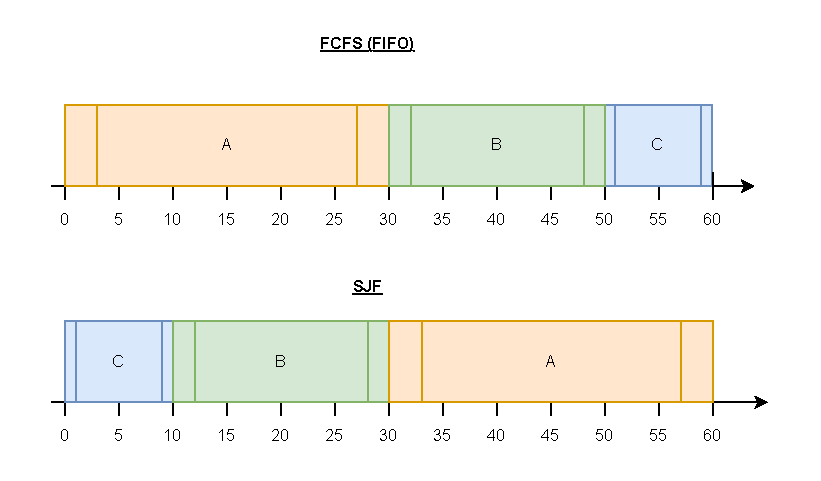
\includegraphics[width=0.9\textwidth]{ej13.pdf}
\end{figure}


\noindent \textit{Ejercicio 14}. Para estos procesos CPU-bound puros dibujar la línea de tiempo y completar la tabla para las políticas apropiativas (con flecha de running a ready): STCF, RR(Q=2). Calcular el promedio de $T_{\text{turnaround}}$ y $T_{\text{response}}$ en cada caso.

\begin{center}
    \begin{tabular}{c|cc|cc|cc}
        Proceso & $T_{\text{arrival}}$ & $T_{\text{CPU}}$ & $T_{\text{firstrun}}$ & $T_{\text{completition}}$ & $T_{\text{turnaround}}$ & $T_{\text{response}}$ \\
        \hline
        A & 2 & 4 & & & & \\
        B & 0 & 3 & & & & \\
        C & 4 & 1 & & & & \\
        \hline
    \end{tabular}
\end{center}

\begin{rta}
    La tabla puede llenarse como:
    \begin{center}
        \begin{tabular}{c|cc|cc|cc}
            Proceso & $T_{\text{arrival}}$ & $T_{\text{CPU}}$ & $T_{\text{firstrun}}$ & $T_{\text{completition}}$ & $T_{\text{turnaround}}$ & $T_{\text{response}}$ \\
            \hline
            A & 2 & 4 & 2 & 7 & 5 & 0 \\
            B & 0 & 3 & 0 & 4 & 4 & 0 \\
            C & 4 & 1 & 6 & 6 & 0 & 2 \\
            \hline
        \end{tabular}
    \end{center}
    Para el diagrama defino la siguiente política: \textbf{cuando hay un empate, se le da prioridad al que lleve mas tiempo en cola}.
\end{rta}

\begin{figure}[h]
    \centering
    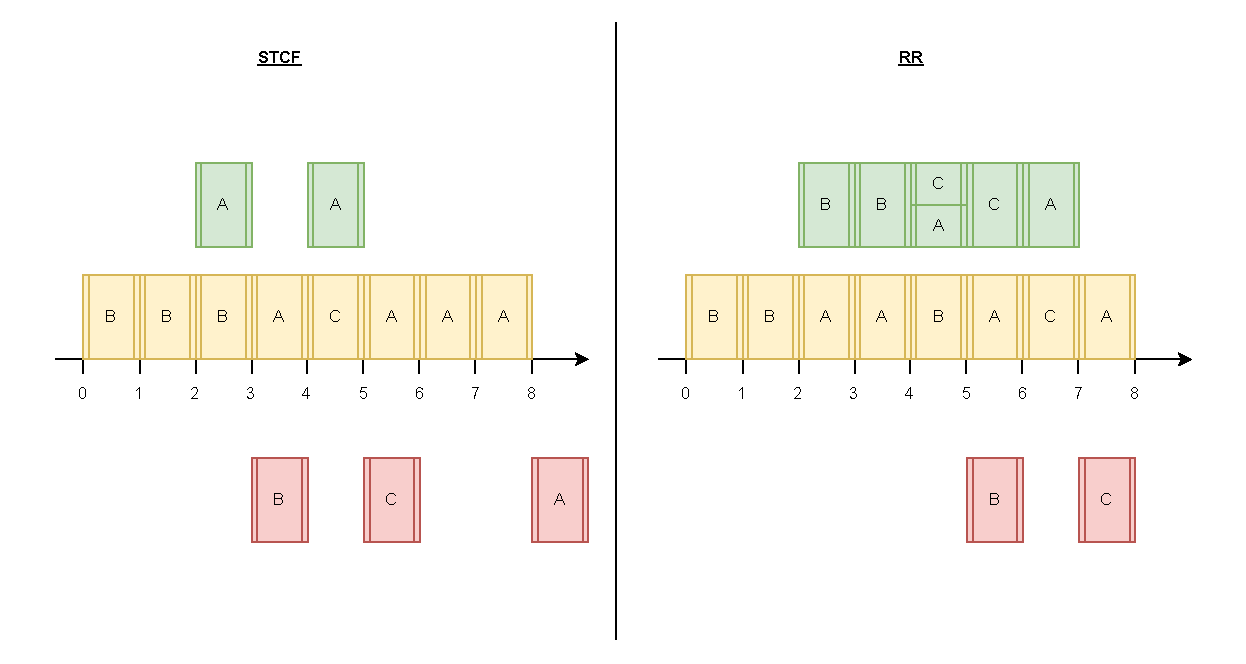
\includegraphics[width=0.9\textwidth]{ej14.pdf}
\end{figure}

\noindent \textit{Ejercicio 15}. Las políticas de planificación se pueden clasificar en dos grades grupos: por lotes (batch) e interactivas. Otra criterio posible es si la planificación necesita el TCP U o no. Clasificar FCFS, SJF, STCF, RR, MLFQ según estos dos criterios.

\begin{rta}
    \begin{itemize}
        \item \textbf{FIFO}: Batch - No necesita TCPU.
        \item \textbf{SJF}: Batch - Sí necesita TCPU.
        \item \textbf{STCF}: 50/50 - Sí necesita TCPU.
        \item \textbf{RR}: Interactiva - No necesita TCPU.
        \item \textbf{MLFQ}: Interactiva - No necesita TCPU.
    \end{itemize}
\end{rta}

\noindent \textit{Ejercicio 16}. Considere los siguientes procesos que mezclan ráfagas de CPU con ráfagas de IO.

\begin{center}
    \begin{tabular}{c|c|ccccccc}
        \rotatebox{90}{Proceso} & \rotatebox{90}{$T_{\text{turnaround}}$} & \rotatebox{90}{$T_{CPU}$} & \rotatebox{90}{$T_{IO}$} & \rotatebox{90}{$T_{CPU}$} & \rotatebox{90}{$T_{IO}$} & \rotatebox{90}{$T_{CPU}$} & \rotatebox{90}{$T_{IO}$} & \rotatebox{90}{$T_{CPU}$} \\
        \hline
        A & 0 & 3 & 5 & 2 & 4 & 1 &   &   \\
        B & 2 & 8 & 1 & 6 &   &   &   &   \\
        c & 1 & 1 & 3 & 2 & 5 & 1 & 4 & 2 \\
        \hline
    \end{tabular}
\end{center}
Realice el diagrama de planificación para un planificador RR (Q=2). Marque bien cuando el proceso está bloqueado esperando por IO.

\begin{rta}
    Asumo la política de que cuando hay dos procesos en cola, tiene mas prioridad el que ya lleve mas tiempo corriendo en el CPU. Los bloques verdes son procesos en \textbf{ready}, los amarillos en \textbf{running} y los rojos \textbf{bloqueados}.
\end{rta}

\begin{figure}[h]
    \centering
    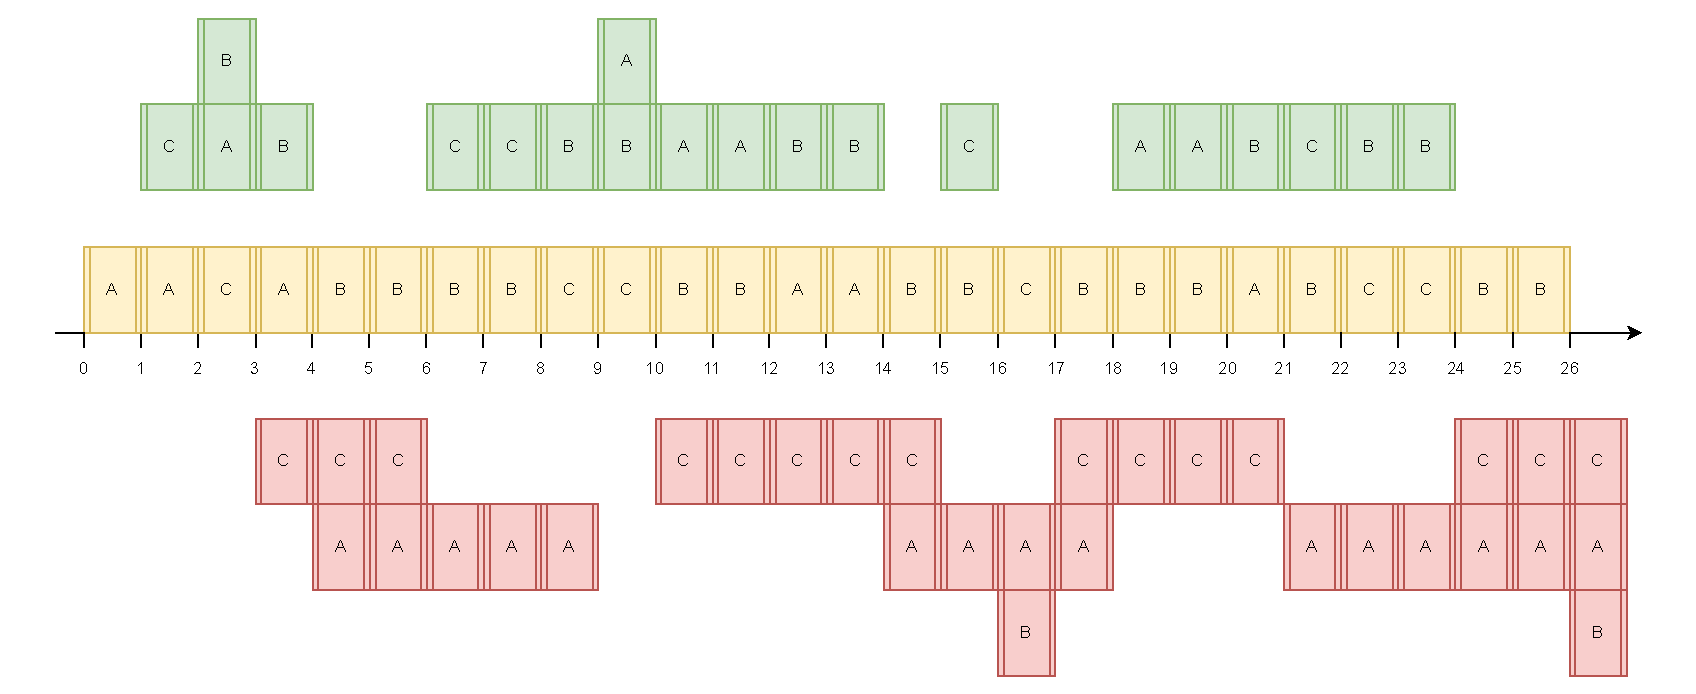
\includegraphics[width=0.9\textwidth]{ej16.pdf}
\end{figure}

\noindent \textit{Ejercicio 17}. Realice el diagrama de planificación para un planificador MLFQ con cuatro colas (Q=1, 2, 4 y 8) para los siguientes procesos CPU-bound:

\begin{center}
    \begin{tabular}{c|cc}
        Proceso & $T_{\text{arrival}}$ & $T_{\text{CPU}}$ \\
        \hline
        A & 0 & 7 \\
        B & 1 & 3 \\
        C & 2 & 4 \\
        D & 4 & 3 \\
        E & 7 & 4 \\
        \hline
    \end{tabular}
\end{center}

\begin{rta}
    Tomando un Quantum de 2, y un segmento de tiempo de 1, el diagrama de planificación sería el siguiente:
\end{rta}
\newpage
\begin{figure}[h]
    \centering
    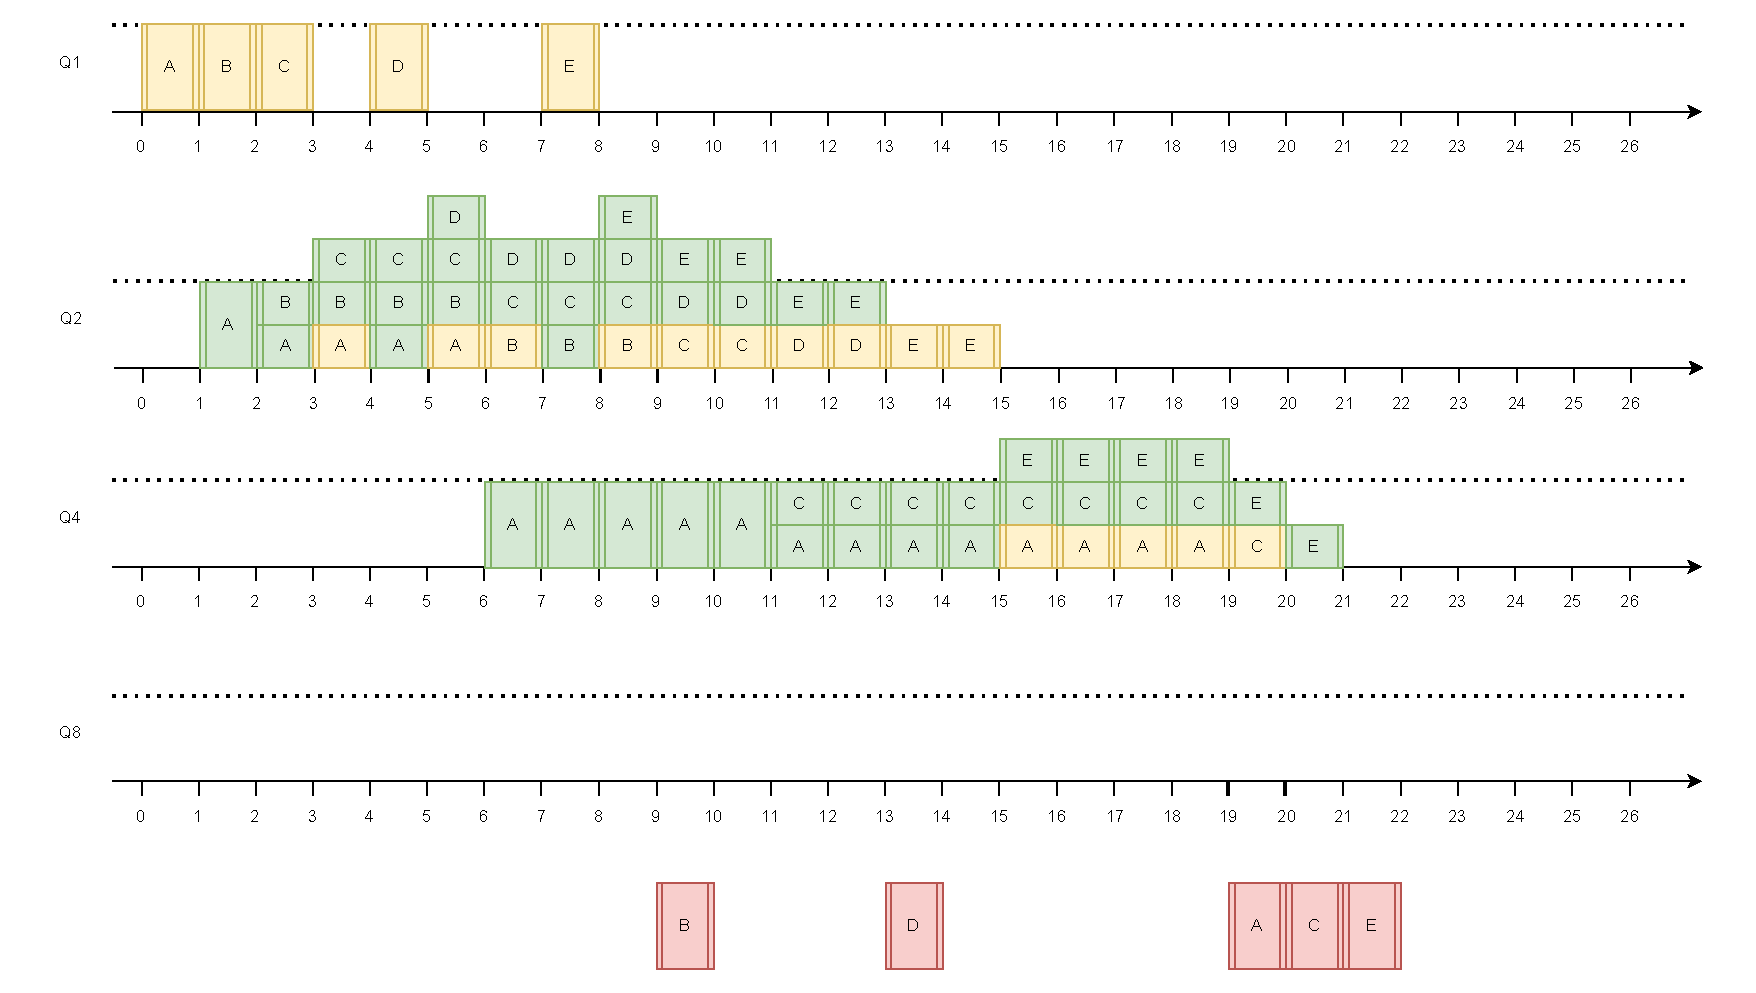
\includegraphics[width=0.9\textwidth]{ej17.pdf}
\end{figure}

\noindent \textit{Ejercicio 18}. Verdadero o falso. Explique.

\begin{itemize}
    \item[(a)] Cuando el planificador es apropiativo (con flecha de Running a Ready) no se puede devolver el control hasta que no pase el quantum.
    \item[(b)] Entre las políticas por lote FCFS y SJF, hay una que siempre es mejor que la otra respecto a $T_\text{turnaround}$.
    \item[(c)] La política RR con quanto = $\infty$ es FCFS.
    \item[(d)] MLFQ sin priority boost hace que algunos procesos puedan sufrir de starvation (inanición). 
    \item[(e)] En MLFQ acumular el tiempo de CPU independientemente del movimiento entre colas evita hacer trampas como \texttt{yield()} un poquitito antes del quantum. 
\end{itemize}

\begin{rta}
    \begin{itemize}
        \item[(a)] Falso, se puede devolver el control por ejemplo cuando se termina el tiempo asignado del proceso.
        \item[(b)] Falso, todo depende del criterio de selección de empate que tomes en FCFS.
        \item[(c)] Verdadero, si el quantum es infinito, entonces el proceso corre hasta que termine.
        \item[(d)] Verdadero, MLFQ sin priority boost puede causar inanición (starvation) porque los procesos de baja prioridad pueden seguir siendo relegados a colas más bajas, mientras que los procesos nuevos o de alta prioridad ocupan los niveles superiores constantemente, impidiendo que los primeros obtengan CPU. 
        \item[(e)] Verdadero, acumular el tiempo de CPU independientemente de los movimientos entre colas previene que los procesos hagan trampas, como llamar a yield() justo antes de que se acabe su quantum para evitar ser movidos a una cola de menor prioridad. Esto ayuda a garantizar un uso justo del CPU.
    \end{itemize}
\end{rta}

\section*{API de Memoria}

\noindent \textit{Ejercicio 1}. Para cada una de las variables de este código indicar si están en el segmento de código,  de pila o de montículo (heap). Si hay punteros indicar a que segmento apunta. \newline
Extra:¿Dónde se ubica el arreglo global si lo declaramos inicializado a cero? int a[N] = \{0\};
\begin{lstlisting}[style=CStyle]
#include <stdlib.h>
#define N 1024

int a[N];
int main(int argc, char ** argv)
{
    int i;
    register int s = 0;
    int *b = calloc(N, sizeof(int));
    for (i=0; i<N; ++i)
        s += a[i]+b[i];
    
    free(b);
    return s;
}    
\end{lstlisting}

\begin{rta}
    \begin{itemize}
        \item \texttt{a} : segmento de datos,
        \item \texttt{b} : stack,
        \item \texttt{\*b} : heap,
        \item \texttt{N} : code,
        \item \texttt{i} : stack,
        \item \texttt{s} : registro de CPU,
        \item \texttt{argc} : stack,
        \item \texttt{argv} : stack.
    \end{itemize}
\end{rta}

\noindent \textit{Ejercicio 2}. Debuggear el mal uso de memoria en los siguientes pedacitos de código.

\begin{lstlisting}[style=CStyle]
char *s = malloc(512);
gets(s);
\end{lstlisting}
\begin{lstlisting}[style=CStyle]
char *s = "Hello Waldo";
char *d = malloc(strlen(s));
strcpy(d,s);
\end{lstlisting}
\begin{lstlisting}[style=CStyle]
char *s = "Hello Waldo";
char *d = malloc(strlen(s));
d = strdup(s);
\end{lstlisting}
\begin{lstlisting}[style=CStyle]
int * a = malloc(16)
a[15] = 42;
\end{lstlisting}

\begin{rta}
    \begin{enumerate}
        \item Uso inseguro de gets, no verifica si se excede el tamaño del buffer ‘s’.
        \item No reserva espacio para el caracter nulo al final de la cadena.
        \item Se pierde la referencia al espacio reservado por malloc.
        \item Asume que los enteros ocupan 1 byte, debería ser \texttt{int * a = malloc(16 * sizeof(int))}.
    \end{enumerate}
\end{rta}

\noindent \textit{Ejercicio 3}. Verdadero o falso. Explique.

\begin{itemize}
    \item[(a)] malloc() es una syscall.
    \item[(b)] malloc() siempre llama a una syscall.
    \item[(c)] malloc() a veces produce una llamada a una syscall.
    \item[(d)] Idem con free().
    \item[(e)] El tiempo de cómputo que toma malloc(x) es proporcional a x.
\end{itemize}

\begin{rta}
    \begin{itemize}
        \item[(a)] Falso. malloc() no es una syscall. Es una librería de C.
        \item[(b)] Falso. Cuando hay memoria disponible en el heap, malloc reutiliza la memoria ya asignada.
        \item[(c)] Verdadero. Si necesita reservar memoria y no hay memoria dinámica libre (y usa la syscall brk)
        \item[(d)] Verdadero. Generalmente la memoria “liberada” pasa a considerarse memoria libre en el heap, sin llamar una syscall necesariamente. Usa brk cuando necesita reducir mucho el tamaño de cierta memoria reservada.
        \item[(e)] Falso. Solo reserva verdaderamente memoria cuando escribo sobre la memoria reservada y solo la necesaria.
    \end{itemize}
\end{rta}

\section*{Traducción de direcciones}
\noindent \textit{Ejercicio 4}. Mostrar la secuencia de accesos a la memoria \textbf{virtual} que se produce al ejecutar este programa assembler x86\_32, donde el registro base=4096 y bounds=256.
\begin{lstlisting}[style=CStyle]
    0: movl $128,%ebx
    5: movl (%ebx),%eax
    8: shll $1, %ebx
    10: movl (%ebx),%eax
    13: retq
\end{lstlisting}

\begin{rta}
    \begin{enumerate}
        \item 0,
        \item 5,
        \item 128,
        \item 8,
        \item 10,
        \item 256,
        \item 13.
    \end{enumerate}
\end{rta}
\section*{Manejo del Espacio Libre}
\noindent \textit{Ejercicio 9}. Suponga un sistema de memoria contiguo con la siguiente secuencia de tamaños de huecos: 10 KiB , $4 \mathrm{KiB}, 20 \mathrm{KiB}, 18 \mathrm{KiB}, 7 \mathrm{KiB}, 9 \mathrm{KiB}, 12 \mathrm{KiB}$, 15 KiB.
Para la siguiente secuencia de solicitudes de segmentos de memoria: 12 KiB , $10 \mathrm{KiB}, 9 \mathrm{KiB}$.\\
¿Cuáles huecos se toman para las distintas políticas?
\begin{itemize}
    \item[(a)] Primer ajuste (first fit).
    \item[(b)] Mejor ajuste (best fit).
    \item[(c)] Peor ajuste (worst fit).
    \item[(d)] Siguiente ajuste (next fit).
\end{itemize}

\begin{rta}
    \begin{itemize}
        \item[(a)] Primer ajuste: 12 KiB en 20 KiB, 10 KiB en 10 KiB, 9 KiB en 18 KiB.
        \item[(b)] Mejor ajuste: 12 KiB en 12 KiB, 10 KiB en 10 KiB, 9 KiB en 9 KiB.
        \item[(c)] Peor ajuste: 12 KiB en 20 KiB, 10 KiB en 18 KiB, 9 KiB en 12 KiB.
        \item[(d)] Siguiente ajuste: 12 KiB en 20 Kib, 10 KiB en 18 KiB, 9 KiB en 9 KiB.
    \end{itemize}
\end{rta}

\newpage
\section*{Paginación}
\noindent \textit{Ejercicio 10}. La TLB de una computadora con una pagetable de un nivel tiene una eficiencia del $95 \%$. Obtener un valor de la TLB toma 10ns. La memoria principal tarda 120ns. ¿Cuál es el tiempo promedio para completar una operación de memoria teniendo en cuenta que se usa tabla de páginas lineal?

\begin{rta}
    Para calcular el tiempo promedio tengo en cuenta lo siguiente, si la TLB falla, es decir en un 0.05 porciento de las veces, va a tener que acceder a la memoria principal por lo que se multiplica por 120ns, en cambio, cuando hace un hit en la TLB, se multiplica por 10ns, ya que al tener los datos en la TLB no necesita acceder a la memoria principal.
    \begin{equation*}
        0.95 \times 10 + 0.05 \times 120 = 14.5 \text{ ns}
    \end{equation*}
\end{rta}

\noindent \textit{Ejercicio 11}. Considere el siguiente programa que ejecuta en un microprocesador con soporte de paginación, páginas de 4 KiB y una TLB de 64 entradas.
\begin{lstlisting}[style=CStyle]
int x[N];
int step = M;
for (int i=0; i<N; i+=step)
    x[i] = x[i]+1;
\end{lstlisting}

\begin{itemize}
    \item[(a)] ¿Qué valores de N, M hacen que la TLB falle en cada iteración del ciclo?
    \item[(b)] ¿Cambia en algo si el ciclo ser repite muchas veces? Explique.
\end{itemize}

\begin{rta}
    Tenemos un arreglo de N enteros de 4 bytes cada uno. Como cada página tiene 4KiB, cada página almacena 1024 enteros. 
    \begin{itemize}
        \item[(a)] Para que la TLB falle en cada iteración del ciclo, el acceso de memoria debería referir a una página que no esté cargada en la TLB, esto sucedería cuando el salto sea demasiado grande. Como cada página tiene 1024 enteros, tomando M>=1024 la TLB fallaría en cada iteración. Pero también hay que tener en cuenta el N, si cada página almacena 1024 palabras y hay 64 entradas en la TLB, basta tomar un N mayor a 64*1024 para que la TLB falle en cada iteración.
        \item[(b)] Cuanto mas se repita el ciclo, mas probable es que la TLB produzca un hit, ya que en cada vuelta del ciclo se accede a las mismas páginas, por lo que la TLB va a tener las páginas cargadas.
    \end{itemize}
\end{rta}

\newpage
\noindent \textit{Ejercicio 12}. Dado un tamaño de página de $4 \mathrm{KiB}=2^{12}$ bytes y la tabla de paginado de la figura.
\begin{itemize}
    \item[(a)] ¿Cuántos bits de direccionamiento hay para cada espacio?
    \item[(b)] Determine las direcciones físicas a partir de las virtuales: 39424, 12416, 26112, 63008, 21760, 32512, 43008, 36096, 7424, 4032.
    \item[(c)] Determine el mapeo inverso, o sea las direcciones virtuales a partir de las direcciones físicas: 16385, 4321.
\end{itemize}

\begin{center}
    \begin{tabular}{|c|c|c|}
    \hline
    V & F & Válida\\
    \hline
    0 & 000 & 1 \\
    \hline
    1 & 111 & 1 \\
    \hline
    2 & 000 & 0 \\
    \hline
    3 & 101 & 1 \\
    \hline
    4 & 100 & 1 \\
    \hline
    5 & 001 & 1 \\
    \hline
    6 & 000 & 0 \\
    \hline
    7 & 000 & 0 \\
    \hline
    8 & 011 & 1 \\
    \hline
    9 & 110 & 1 \\
    \hline
    10 & 100 & 1 \\
    \hline
    11 & 000 & 0 \\
    \hline
    12 & 000 & 0 \\
    \hline
    13 & 000 & 0 \\
    \hline
    14 & 000 & 0 \\
    \hline
    15 & 010 & 1 \\
    \hline
    \end{tabular}
    \end{center}

\begin{rta}
    \begin{itemize}
        \item[(a)] Para \textbf{Virtual}: 16 bits. 
        \begin{itemize}
            \item 4 bits para la VPN (la tabla tiene 16 entradas).
            \item 12 bits para el offset.
        \end{itemize}
        Para \textbf{Físico}: 15 bits.
        \begin{itemize}
            \item 3 bits para PFN. 
            \item 12 bits para el offset.
        \end{itemize}
        \item[(b)] Para traducir de virtual a física se hace lo siguiente:
        \begin{enumerate}
            \item Divido la dirección virtual en VPN y offset.
            \item Con el VPN busco en la tabla de páginas y obtengo el PFN.
            \item Lo convinado con el offset para obtener la dirección física.
        \end{enumerate}
        \begin{itemize}
            \item 39424 = $(1001101000000000)_{2}$
            \begin{itemize}
                \item VPN = 1001 = 9
                \item Offset = 101000000000.
                \item PFN = 110 = 6
                \item Dirección física = 110101000000000. = 0x6A00 = 27136.
            \end{itemize}
            \item 12416 = $(11000010000000)_2$
            \begin{itemize}
                \item VPN = 1100 = 12
            \end{itemize}
            La entrada es inválida, no hay mapeo.
            \item 26112 = $(110011000000000)_2$
            \begin{itemize}
                \item VPN = 1100 = 12
            \end{itemize}
            La entrada es inválida, no hay mapeo.
            \item 63008 = $(1111011000100000)_2$
            \begin{itemize}
                \item VPN = 1111 = 15
                \item Offset = 011000100000.
                \item PFN = 010 = 2
                \item Dirección física = 010011000100000 = 0x2620 = 9760.
            \end{itemize}
        \end{itemize}
        \item[(c)] Para mapear de físico a virtual se hace lo siguiente:
        \begin{enumerate}
            \item Divido la dirección física en PFN y offset.
            \item Busco el PFN en la tabla de páginas y obtengo el VPN.
            \item Con el VPN y el offset obtengo la dirección virtual.
        \end{enumerate}
        \begin{itemize}
            \item 16385 = $(100000000000001)_2$
            \begin{itemize}
                \item PFN = 100
                \item Offset = 000000000001.
                \item VPN = 4
                \item Dirección virtual = 0100000000000001 = 0x4001 = 16385
            \end{itemize}
        \end{itemize}
    \end{itemize}
\end{rta}

\newpage
\noindent \textit{Ejercicio 13}. Dado el siguiente esquema de paginación i386 (10, 10, 12) traducir la direcciones virtuales 0x003FF666, 0x00000AB0, 0x00800B0B a físicas.

\begin{figure}[h]
    \centering
    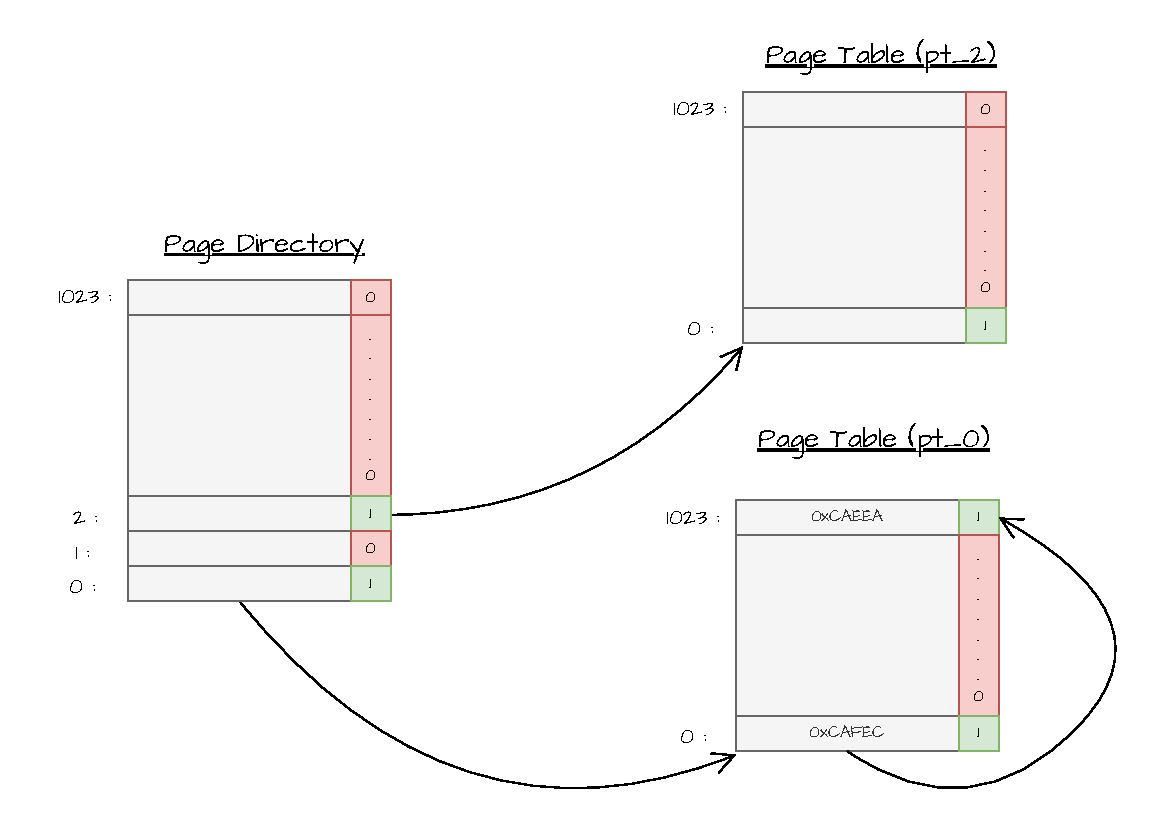
\includegraphics[width=0.5\textwidth]{ej131.pdf}
\end{figure}

\begin{rta}
    En el dibujo mas abajo, las flechas rojas indican el mapeo de las direcciones virtuales a las direcciones físicas.
    \begin{itemize}
        \item 0x003FF666 = la dirección física a la que mapea es 0xCAEEA666, entrada 1023 de la page table 0, con un offset de 666.
        \item 0x00000AB0 = la dirección física a la que mapea es 0xCAFECAB0, entrada 0 de la page table 0, con un offset de AB0.
        \item 0x00800B0B = la dirección física a la que mapea es la que esté presente en la entrada 0 de la page table 2, (se olvidaron de escribir la dirección).
    \end{itemize}
\end{rta}

\begin{figure}[h]
    \centering
    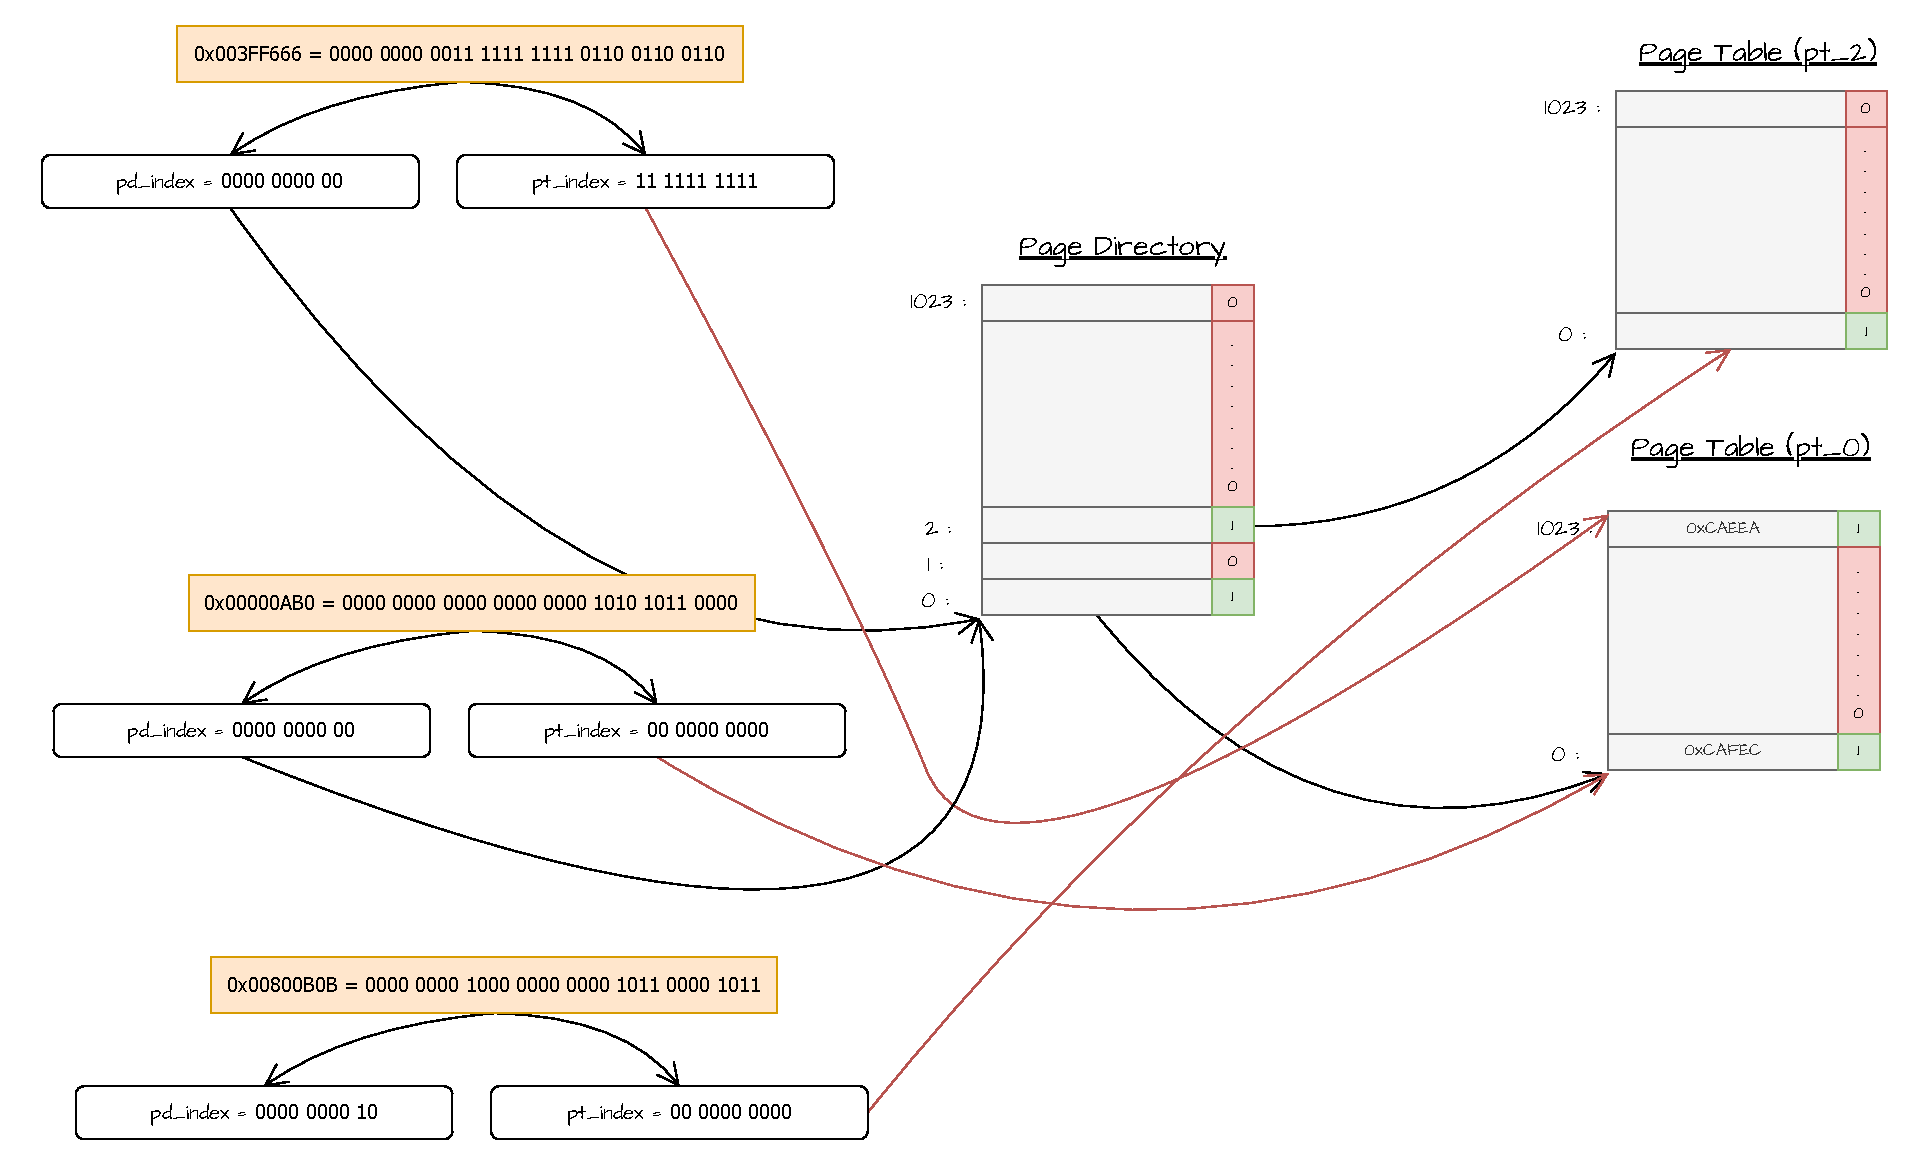
\includegraphics[width=0.7\textwidth]{ej132.pdf}
\end{figure}


\newpage
\noindent \textit{Ejercicio 14}. Dado el sistema de paginado de dos niveles del i386 direcciones virtuales de 32 bits, direcciones físicas de 32 bits, 10 bits de índice de page directory, 10 bits de índice de table directory, y 12 bits de offset dentro de la página, o sea un $(10,10,12)$, indicar:
\begin{itemize}
    \item[(a)] Tamaño de total ocupado por el directorio y las tablas de página para mapear 32 MiB al principio de la memoria virtual.
    \item[(b)] Tamaño total del directorio y tablas de páginas si están mapeados los 4 GiB de memoria.
    \item[(c)] Dado el ejercicio anterior ¿Ocuparía menos o más memoria si fuese una tabla de un solo nivel? Explicar.
    \item[(d)] Mostrar el directorio y las tablas de página para el siguiente mapeo de virtual a física:
\end{itemize}

\begin{center}
\begin{tabular}{r|r}
Virtual & Física \\
\hline
$[0 M i B, 4 M i B)$ & $[0 M i B, 4 M i B]$ \\
$[8 M i B, 8 M i B+32 K i B)$ & $[128 M i B, 128 M i B+32 K i B)$ \\
\end{tabular}
\end{center}

\begin{figure}[h]
    \centering
    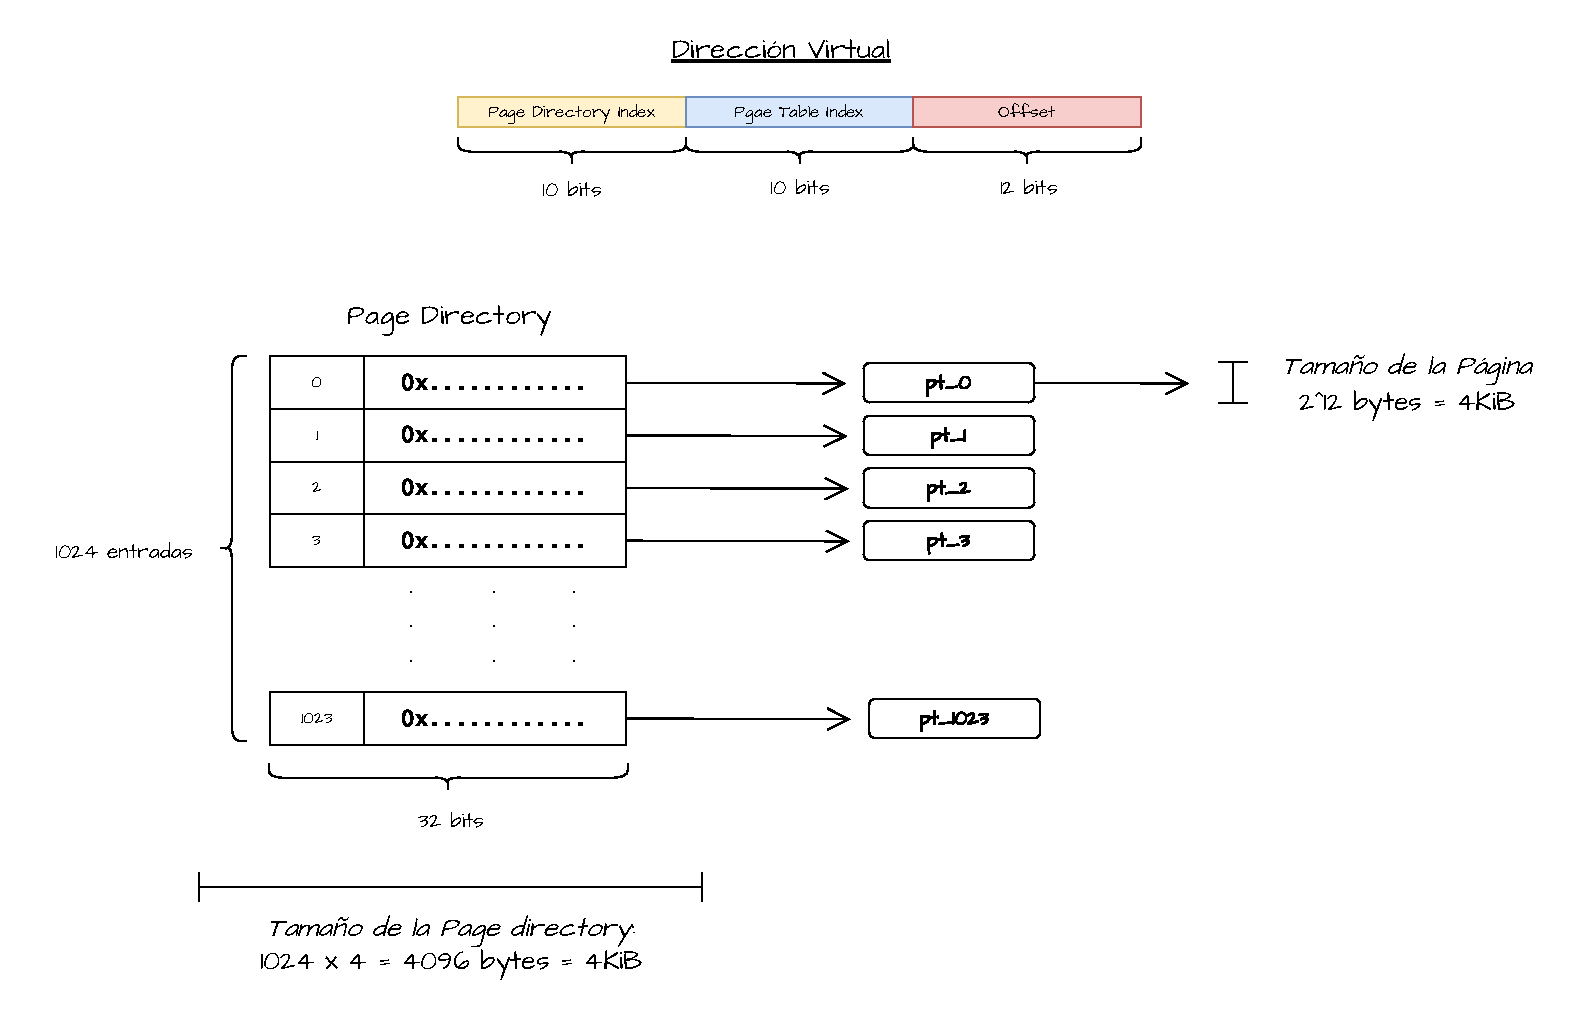
\includegraphics[width=1\textwidth]{ej142.pdf}
\end{figure}

\newpage
\begin{rta}
    \begin{itemize}
        \item[(a)] Viendo la distribución de la memoria, se puede ver que se va a necesitar por un lado los 4KiB de la \textbf{Page Directory} y por otro lado la cantidad de páginas que se usen en la cantidad buscada:
        \begin{equation*}
            \frac{32MiB}{4KiB} = \frac{2^{25}}{2^{12}} = 2^{13} = 8192 \text{ páginas}
        \end{equation*}
        Como cada \textbf{page table} apunta a 1024 páginas físicas, se necesitan 8 \textbf{page tables} para mapear 32MiB. Entonces el total ocupado por el directorio y las tablas de página es:
        \begin{equation*}
            4KiB + 8 \times 4KiB = 36KiB
        \end{equation*}
        \item[(b)] Si están mapeados los 4GiB de memoria, quiere decir que se tienen una cantidad de páginas de:
        \begin{equation*}
            \frac{4GiB}{4KiB} = \frac{2^{32}}{2^{12}} = 2^{20} = 1048576 \text{ páginas}
        \end{equation*}
        Como cada \textbf{page table} apunta a 1024 páginas físicas, se necesitan 1024 \textbf{page tables} para mapear 4GiB. Entonces el total ocupado por el directorio y las tablas de página es:
        \begin{equation*}
            4KiB + 1024 \times 4KiB = 4KiB + 4MiB = 2^{12} + 2^{22} = 4198400 \text{ bytes} = 4100KiB
        \end{equation*}
        \item[(c)] Si fuese una tabla de un solo nivel, se necesitaría menos memoria, ya que no se tendría que mantener un espacio para la \textbf{Page Directory}, sino que se tendría que mantener un espacio para las 1048576 páginas.
        \item[(d)] El gráfico muestra el mapeo de virtual a física. Se puede ver que:
        \begin{itemize}
            \item El primer rango de direcciones virtuales va a mapear la \textbf{page table} completa que esta apuntada por la entrada 0 del \textbf{page directory}.
            \item El segundo rango de direcciones virtuales va a mapear una \textbf{page table} con 8 entradas válidas y el resto inválidas. Esta tabla esta apuntada por la entrada 2 del \textbf{page directory}.
        \end{itemize}
    \end{itemize}
\end{rta}

\begin{figure}[h]
    \centering
    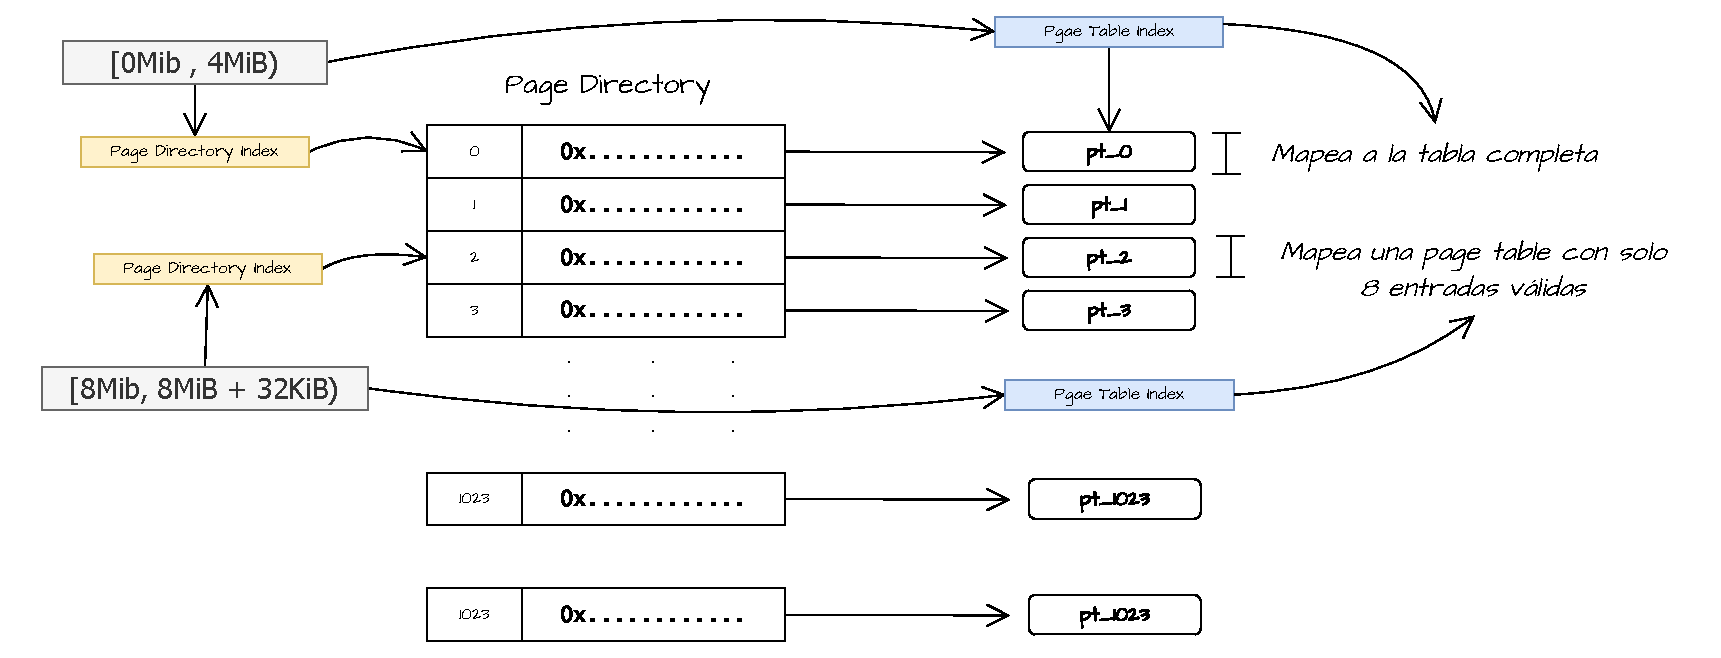
\includegraphics[width=1\textwidth]{ej143.pdf}
\end{figure}

\newpage
\noindent \textit{Ejercicio 15}.  Explique porque un i386 no puede mapear los 4 GiB completos de memoria virtual. ¿Cuál es el máximo?

\begin{rta}
    Esto se debe a que los metadatos ocupan espacio, y en el caso de un i386, tenemos los 4GiB de memoria total.
\end{rta}

\noindent \textit{Ejercicio 16}. Explique como podría extender el esquema de memoria virtual del i386 para que, aunque cada proceso tenga acceso a 4 GiB de memoria virtual (32 bits), en total se puedan utilizar 64 GiB (36 bits) de memoria física.

\begin{rta}
    Se podría extender el esquema de memoria virtual del i386 para que, aunque cada proceso tenga acceso a 4 GiB de memoria virtual (32 bits), en total se puedan utilizar 64 GiB (36 bits) de memoria física, utilizando un esquema de paginación de tres niveles. Con el formato \textbf{(2,9,9,12)} donde se tenga lo siguiente:
    \begin{itemize}
        \item CR3 apunta a la \textbf{Page Directory Pointer Table} (PDPT) de 4 entradas con 2 bits de direccionamiento.
        \item Una \textbf{page directory} de 512 entradas con 9 bits de direccionamiento.
        \item Con \textbf{page tables} de 512 entradas con 9 bits de direccionamiento.
    \end{itemize} 
\end{rta}

\noindent \textit{Ejercicio 17}. ¿Verdadero o Falso? Explique.
\begin{itemize}
    \item[(a)] Hay una page table por cada proceso.
    \item[(b)] La MMU siempre mapea una memoria virtual más grande a una memoria física más pequeña. 
    \item[(c)] La dirección física siempre la entrega la TLB. 
    \item[(d)] Dos páginas virtuales de un mismo proceso se pueden mapear a la misma página física. 
    \item[(e)] Dos páginas físicas de un mismo proceso se pueden mapear a la misma página virtual.
    \item[(f)] En procesadores de 32 bits y gracias a la memoria virtual, cada proceso tiene $2^{32}$ direcciones de memoria.
    \item[(g)] La memoria virtual se puede usar para ahorrar memoria.
    \item[(h)] Toda la memoria virtual tiene que estar mapeada a memoria física.
    \item[(i)] El page directory en i386 se comparte entre todos los procesos.
    \item[(j)] Puede haber marcos de memoria física que no tienen un marco de memoria virtual que los apunte. 
    \item[(k)] Por culpa de la memoria virtual hacer un \texttt{fork} resulta muy caro en términos de memoria.
    \item[(l)] Los procesadores tienen instrucciones especiales para acceder a la memoria física evitando la MMU. 
    \item[(m)] Es imposible hacer el mapeo inverso de física a virtual.
    \item[(n)] No se puede meter un todo un Sistema Operativo completo con memoria paginada i386 en 4 KiB.
\end{itemize}

\begin{rta}
    \begin{itemize}
        \item[(a)] Verdadero.
        \item[(b)] Falso. Va a depender de lo que demande el proceso.
        \item[(c)] Verdadero.
        \item[(d)] Verdadero.
        \item[(e)] Falso. Cada página física se mapea a una única página virtual, no sería función de mapeo.
        \item[(f)] Verdadero.
        \item[(g)] Verdadero.
        \item[(h)] Falso.
        \item[(i)] Falso. Hay un pagedir (PD) por cada proceso. Justamente cambiar de contexto es apuntar el CR3 a la dirección física de ese PD.       
        \item[(j)] Verdadero. Es posible que haya marcos de direccion virtual sin un marco fisico asociado, podria ser porque no estan siendo utilizados o bien porque el MMU todavia no les asigno un marco fisico.
        \item[(k)] Falso. Gracias a la memoria virtual hacer un fork resulta tremendamente barato utilizando el metodo CoW (Copy on Write).  
        \item[(l)] Falso. Una vez que se entra a la memoria virtual no se puede salir, todo se maneja a través de la MMU.
        \item[(m)] Falso. Es posible tanto mapear memoria fisica a virtual como virtual a fisica y esto se llama \textbf{page walking}.
        \item[(n)] Falso. Es posible utilizando recursión introducir todo un sistema operativo en una sola entrada de PD    
    \end{itemize}
\end{rta}


\newpage
\noindent \textit{Ejercicio 18}. Se define un page directory donde la última entrada, la 1023, apunta a la base del
mismo

\begin{itemize}
    \item[(a)] ¿A dónde apunta la dirección virtual 0xFFC00000?
    \item[(b)] ¿Y la dirección virtual 0xFFFE0000?
    \item[(c)] Indique a donde apunta la dirección virtual 0xFFFFF000.
    \item[(d)] Finalmente, describa para que sirve este esquema de memoria virtual.
\end{itemize}

\begin{figure}[h]
    \centering
    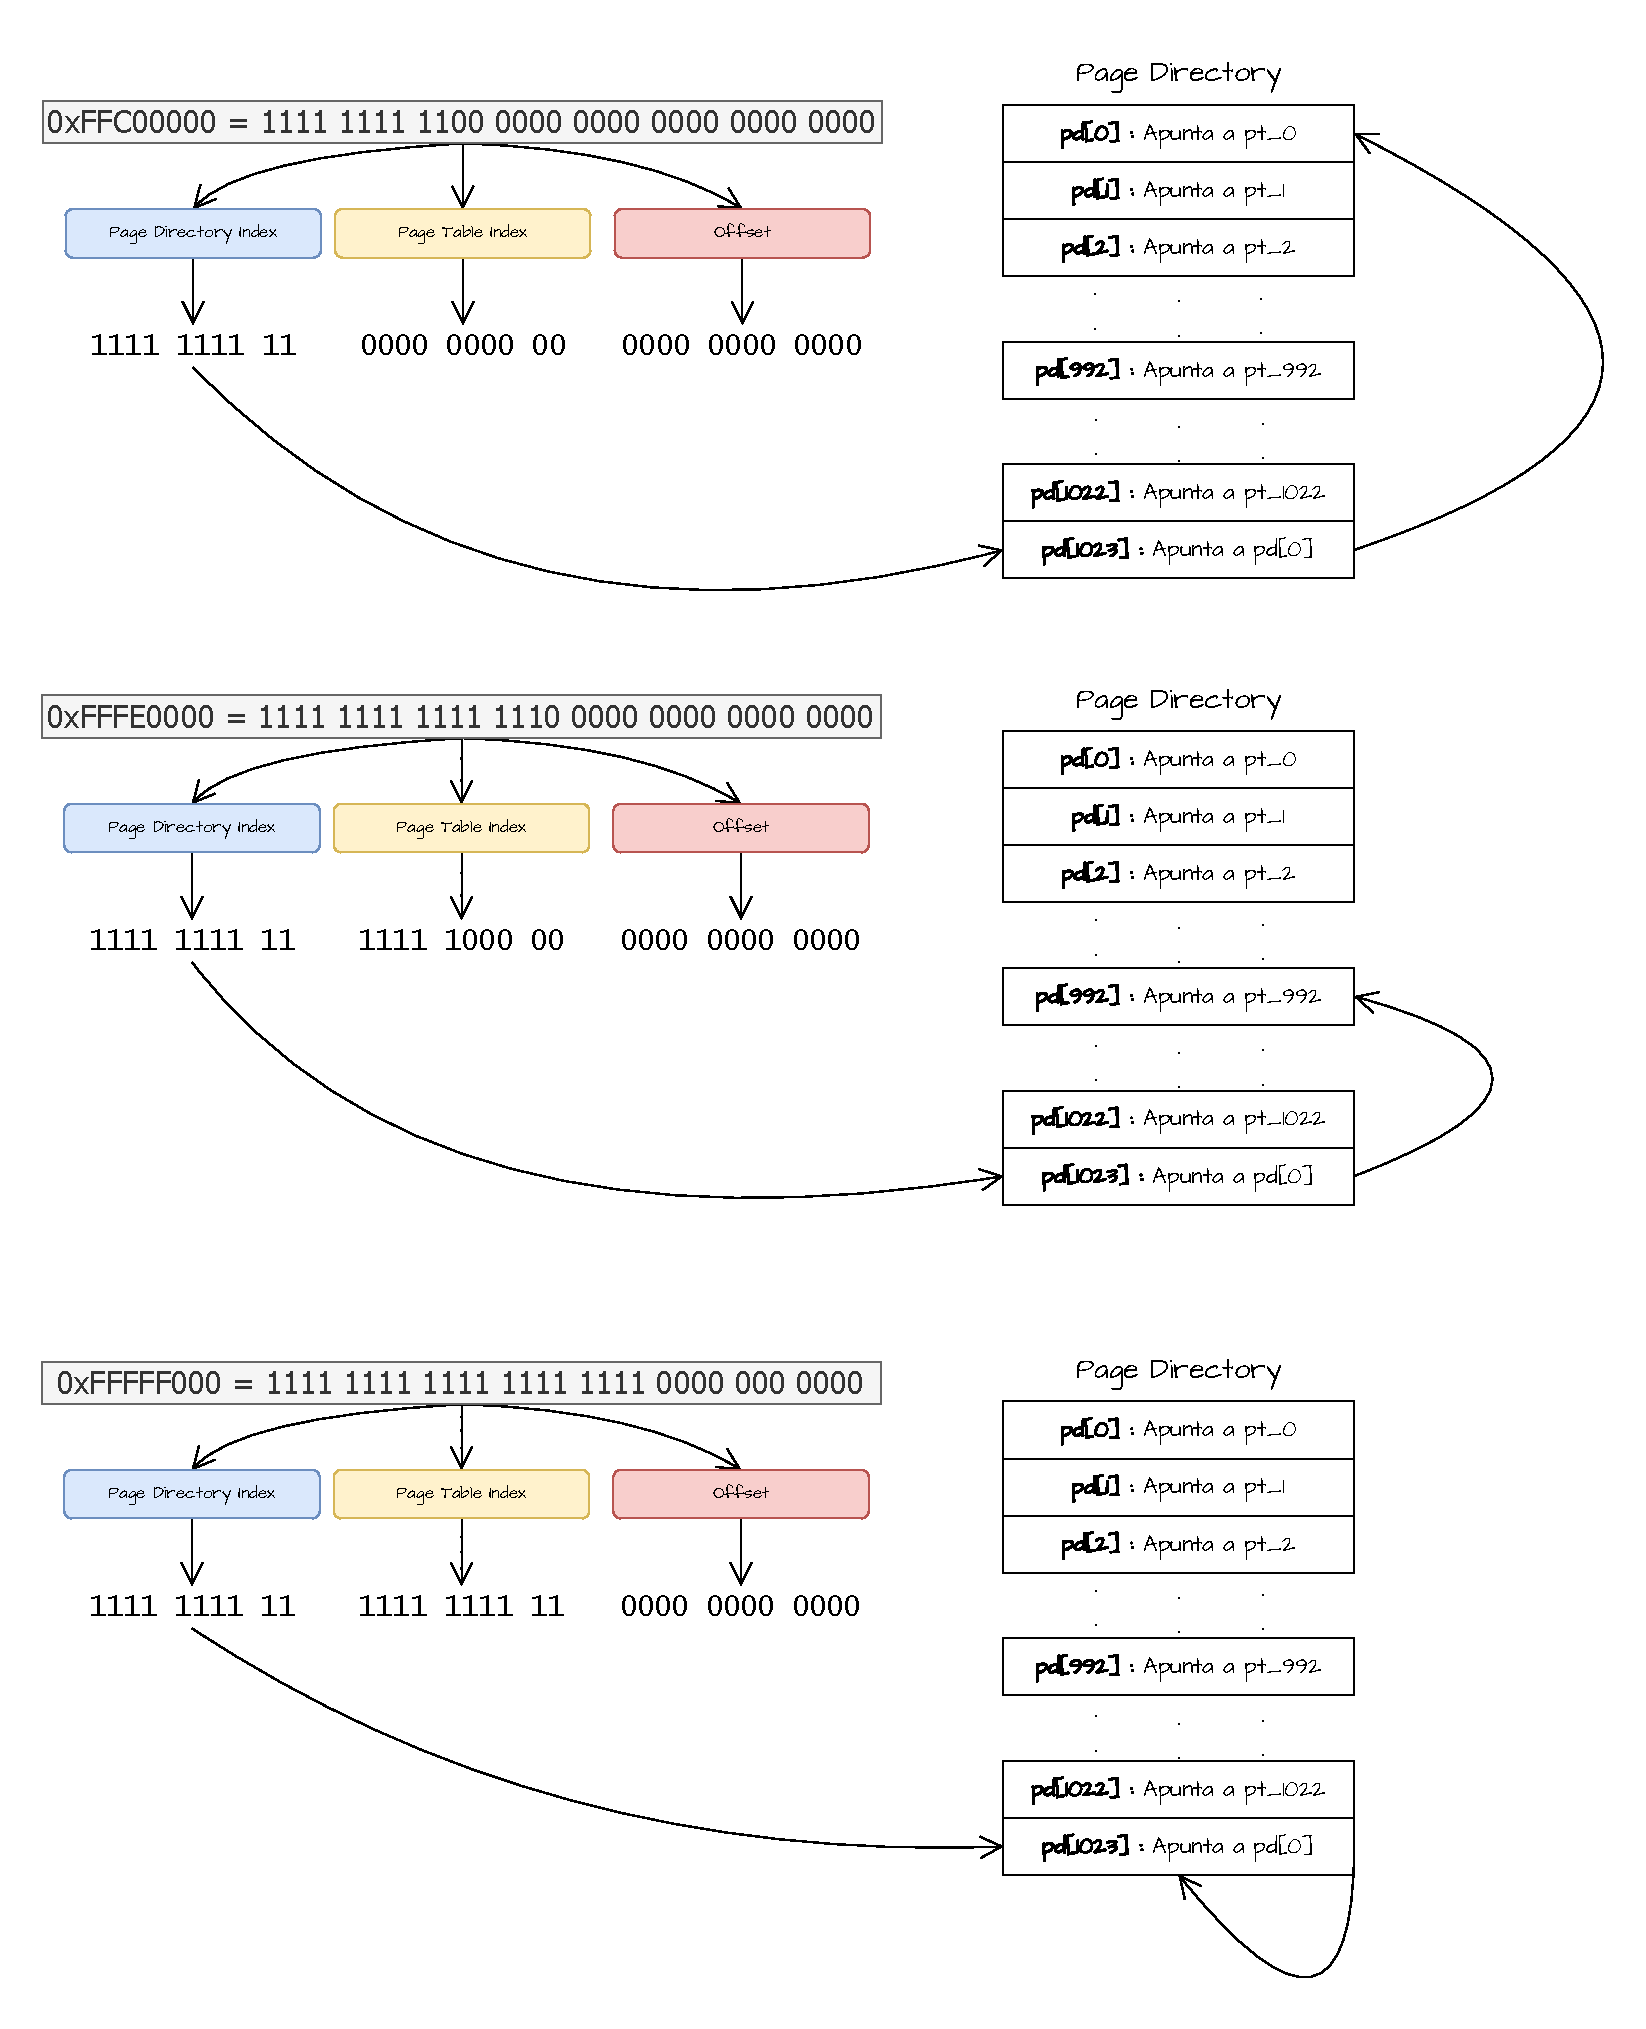
\includegraphics[width=0.83\textwidth]{ej18.pdf}
\end{figure}

\begin{rta}
    \begin{itemize}
        \item[(a)] Como se ve en el diagrama, la dirección virtual 0xFFC00000 apunta a si mísma, ya que es la última entrada de la page directory. Entonces debo mirar la page directory como si fuese una page table, ir a la primera entrada, y de alli conluyo que con la dirección 0xFFC00000 puedo ver todo lo que contiene la primera page table. 
        \item[(b)] La dirección virtual 0xFFFE0000 se indexa en 0xFFC00000 que apunta a si mísma, ya que es la última entrada de la page directory. Entonces debo mirar la page directory como si fuese una page table, ir a la primera entrada, y de alli conluyo que con la dirección 0xFFFE0000 puedo ver todo lo que contiene la page table 992.
        \item[(c)] Con la dirección virtual 0xFFFFF000 puedo ver todo lo que contiene la page directory, ya que veo lo que tiene la page table en la entrada 1023, y esta apunta a la base de la page directory. Es una forma de ver toda la estructura.
        \item[(d)] Este esquema de memoria me facilita mapear toda la estructura del page directory y todas las page tables en memoria virtual.
    \end{itemize}
\end{rta}

\noindent \textit{Ejercicio 19}. Explique como se usa la paginación para hacer:

\begin{itemize}
    \item[(a)] Dereferenciamiento de puntero a \textit{NULL} tira excepción.
    \item[(b)] Archivo de intercambio o \textit{swap file}.
    \item[(c)] \textit{Demand paging} para la carga de programas.
    \item[(d)] Auto-growing stack.
    \item[(e)] Non-executable stacks.
    \item[(f)] Memory mapped files \texttt{mmap()}.
    \item[(g)] Copy-on-write (COW) para el \textit{fork()}.
    \item[(h)] \texttt{sbrk()} barato y por lo tanto \texttt{malloc()} barato.
    \item[(i)] \texttt{malloc()}; \texttt{memset(0) = calloc()} barato.
    \item[(j)] Código compartido entre procesos: shared libraries, código de kernel, etc. 
    \item[(k)] Memoria compartida entre procesos. 
\end{itemize}

\begin{rta}
    \begin{itemize}
        \item[(a)] Dereferenciamiento de puntero a \textit{NULL} tira excepción: En alguna dirección del espacio virtual se le deja reservado para NULL, con ninguna dirección física asignada, por lo que al intentar acceder a esa dirección se produce una excepción.
        \item[(b)] Archivo de intercambio o \textit{swap file}: cuando una página no se ha usado recientemente, se marca como "no residente" y se escribe en el archivo de intercambio. Si esa página es requerida nuevamente, se genera una falla de página y el sistema la carga desde el archivo de intercambio de vuelta a la memoria física.
        \item[(c)] \textit{Demand paging} para la carga de programas: se carga unicamente las paginas necesarias para correr el programa y en el momento que el programa quiere acceder a una pagina que no estaba cargada ocurre un page fault.
        Al ocurrir un page fault cuando el programa necesitaba acceder a una página que no está actualmente en la memoria, el sistema operativo carga las páginas requeridas del disco en la memoria y actualiza las page tables. Este proceso es transparente para el programa en ejecución y continúa ejecutándose como si la página siempre hubiera estado en la memoria.  
        \item[(d)] Auto-growing stack:  si el proceso accede a una dirección que está justo fuera del espacio actual del stack, se genera una falla de página. El sistema operativo detecta que la página faltante es parte del crecimiento del stack y asigna una nueva página para ampliar el stack automáticamente.
        \item[(e)] Non-executable stacks: se agrega un bit en las entradas de la tabla de páginas, lo que previene que se ejecute código en esas páginas. Esto es útil para evitar ciertos tipos de ataques, como la inyección de código en el stack.
        \item[(f)] Memory mapped files \texttt{mmap()}: Cuando el proceso accede a una parte del archivo mapeado, el sistema operativo asigna las páginas físicas correspondientes y carga el contenido del archivo en esas páginas, permitiendo el acceso directo al archivo como si fuera memoria.
        \item[(g)] Copy-on-write (COW) para el \textit{fork()}: la idea detrás de CoW es que cuando un proceso padre crea un proceso hijo, ambos procesos inicialmente compartirán las mismas páginas en la memoria y estas páginas compartidas se marcarán como copy-on-write, lo que significa que, si las hay, de estos procesos intentará modificar las páginas compartidas, entonces solo se creará una copia de estas páginas y las modificaciones se realizarán en la copia de las páginas por ese proceso y, por lo tanto, no afectarán al otro proceso.  
        \item[(h)] \texttt{sbrk()} barato y por lo tanto \texttt{malloc()} barato: el crecimiento del heap no implica una asignación física inmediata de páginas. Las páginas solo se asignan cuando el proceso realmente intenta usarlas, haciendo que operaciones como malloc() sean más eficientes al principio, ya que solo se asignan páginas físicas cuando es necesario.
        \item[(i)] \texttt{malloc()}; \texttt{memset(0) = calloc()} barato: Cuando se asigna memoria con calloc(), el sistema puede simplemente asignar páginas de manera diferida y marcar las páginas como compartidas entre los procesos que las necesitan. Las páginas se inicializan en 0 solo cuando se acceden por primera vez, usando copy-on-write.
        \item[(j)] Código compartido entre procesos: shared libraries, código de kernel, etc.: varias entradas en la tabla de páginas de diferentes procesos pueden apuntar a las mismas páginas físicas, permitiendo que múltiples procesos compartan el mismo código, ahorrando memoria.
        \item[(k)] Memoria compartida entre procesos: el sistema operativo puede permitir que dos o más procesos compartan ciertas áreas de memoria. Esto se hace mapeando las mismas páginas físicas en el espacio de direcciones virtuales de diferentes procesos. Las tablas de páginas se configuran de modo que ambos procesos accedan a la misma memoria física, permitiendo la comunicación entre ellos sin copias adicionales. 
    \end{itemize}
\end{rta}


\end{document}
